\section{The graded loophole: supersymmetry in eight dimensions}
\label{sec:susy}

\subsection{The super-Poincar\'e algebras}

The one extension of the conclusion of Coleman and Mandula that survives all their hypotheses is a
superalgebra~\cite{HLS1975,Nahm1978,Strathdee1987}. We build it explicitly on both spacetimes, with
the matrices of the project. Its generators are the 28 Lorentz generators $\mathcal J^{AB}_{\rm NG}$
($A<B$), the 8 momenta $\mathcal P^{\rm NG}_C$, 16 supercharges $\mathcal Q^{\rm NG}_l$ ($l=1,\dots,16$, one
for each real spinor component), and an R-charge $\mathcal R_{\rm NG}$. With the metric
$\eta_{\rm NG}$ of the spacetime (diagonal, entries $\eta_{AA}^{\rm NG}=\pm1$), the nonzero brackets are
\begin{subequations}
\label{eq:superalgebra}
\begin{align}
[\mathcal J^{AB}_{\rm NG},\mathcal J^{CD}_{\rm NG}]&=\eta^{\rm NG}_{BC}\mathcal J^{AD}_{\rm NG}-\eta^{\rm NG}_{AC}\mathcal J^{BD}_{\rm NG}\nonumber\\
&\quad-\eta^{\rm NG}_{BD}\mathcal J^{AC}_{\rm NG}+\eta^{\rm NG}_{AD}\mathcal J^{BC}_{\rm NG},\\
[\mathcal J^{AB}_{\rm NG},\mathcal P^{\rm NG}_C]&=\eta^{\rm NG}_{BC}\mathcal P^{\rm NG}_A-\eta^{\rm NG}_{AC}\mathcal P^{\rm NG}_B,\\
[\mathcal J^{AB}_{\rm NG},\mathcal Q^{\rm NG}_l]&=\sum_{l'}(\Sigma^{\rm NG}_{AB})_{l'l}\,\mathcal Q^{\rm NG}_{l'},\\
\{\mathcal Q^{\rm NG}_l,\mathcal Q^{\rm NG}_{l'}\}&=\sum_C(\mathsf Y^C_{\rm NG})_{ll'}\,\mathcal P^{\rm NG}_C,\\
[\mathcal R_{\rm NG},\mathcal Q^{\rm NG}_l]&=\sum_{l'}(\omega_{\rm NG})_{l'l}\,\mathcal Q^{\rm NG}_{l'},
\end{align}
\end{subequations}
where $\mathcal J^{BA}_{\rm NG}=-\mathcal J^{AB}_{\rm NG}$ and $\mathcal J^{AA}_{\rm NG}=0$, the spinor generators
with lowered indices are $\Sigma^{\rm NG}_{AB}=\eta^{\rm NG}_{AA}\eta^{\rm NG}_{BB}\Sigma^{AB}_{\rm NG}$, and the
matrices of the anticommutator are $\mathsf Y^C_{\rm NG}=2C^+_{\rm NG}\gamma^C_{\rm NG}$. On both spacetimes
$C^+_{\rm NG}\gamma^C_{\rm NG}(C^+_{\rm NG})^{-1}=(\gamma^C_{\rm NG})^T$ and $C^+_{\rm NG}$ is symmetric, so every
$\mathsf Y^C_{\rm NG}$ is symmetric, as an anticommutator requires; the R-charge acts through
$\omega_{\rm NG}=\gamma^0_{\rm NG}\cdots\gamma^7_{\rm NG}$, which commutes with every
$\gamma^A_{\rm NG}\gamma^B_{\rm NG}$, so $\mathcal R_{\rm NG}$ commutes with $\mathcal J^{AB}_{\rm NG}$ and
$\mathcal P^{\rm NG}_C$: it is an internal symmetry. It does not commute with the supercharges, and their
anticommutator is a momentum. Lorentz and internal symmetry are tied together through the odd
generators.

The program builds the complete table of brackets of the 53 generators and checks the graded Jacobi
identity, $(-1)^{|\mathsf x||\mathsf z|}[\mathsf x,[\mathsf y,\mathsf z]\}+\text{cyclic}=0$ with $|\mathsf x|=1$ for a
supercharge and 0 otherwise, on every one of the {{GEN:susy_triples}} ordered triples of generators,
on both spacetimes: no triple violates it (checks S-1, S-2a). All structure constants are integers,
halves or quarters; binary floating-point arithmetic represents them and all their sums and
products exactly, so the check is exact.

\subsection{Positivity: present on 7+1, absent on 4+4}

For Hermitian supercharges the matrix $\{\mathcal Q^{\rm NG}_l,\mathcal Q^{\rm NG}_{l'}\}$ has a nonnegative
expectation value in every state, because $\langle\{\mathcal Q^{\rm NG}_{\mathsf v},\mathcal Q^{\rm NG}_{\mathsf v}\}\rangle=
2\lVert\mathcal Q^{\rm NG}_{\mathsf v}\lvert\cdot\rangle\rVert^2$ for every real combination $\mathcal Q^{\rm NG}_{\mathsf v}=\sum_l\mathsf v^l\mathcal Q^{\rm NG}_l$ of them (with real coefficients $\mathsf v^l$ and any state $\lvert\cdot\rangle$).
On $7+1$, $C^+_{1671}\gamma^4_{1671}=\mathsf 1_{16}$, and the seven matrices $C^+_{1671}\gamma^A_{1671}$ with
$A\neq4$ anticommute and square to $\mathsf 1_{16}$ (check S-4). Hence
$\sum_C\mathsf Y^C_{\rm NG}\mathcal P^{\rm NG}_C$ has the eigenvalues
$2(\mathcal P^{\rm NG}_4\pm\lvert\vec{\mathcal P}_{\rm NG}\rvert)$, with $\lvert\vec{\mathcal P}_{\rm NG}\rvert^2=
\sum_{A\neq4}(\mathcal P^{\rm NG}_A)^2$: it is positive exactly for momenta in the forward light cone, and
unitary representations of positive energy exist. The R-symmetry is compact: $\omega_{1671}^2=
-\mathsf 1_{16}$, so $\exp(\varphi_{\rm NG}\omega_{1671})=\cos\varphi_{\rm NG}+\omega_{1671}\sin\varphi_{\rm NG}$ is a rotation by an
angle $\varphi_{\rm NG}$, a group $U(1)$. This is the minimal supersymmetry algebra of eight dimensions, with 16 real
supercharges~\cite{Strathdee1987,KugoTownsend1983}.

On $4+4$ every $\mathsf Y^C_{\rm NG}=2C^+_{1644}\gamma^C_{1644}$ is traceless (a product of an odd number of
different Dirac matrices), so $\sum_C\mathsf Y^C_{\rm NG}\mathcal P^{\rm NG}_C$ is traceless and nonzero for
every nonzero momentum and has a negative eigenvalue (check S-4, Fig.~\ref{fig:susy}): the algebra
exists, its Jacobi identities hold, but it has no unitary representation with nonzero momentum
(hypothesis H8 fails). Its R-symmetry is non-compact, $\omega_{1644}^2=+\mathsf 1_{16}$, and
$\exp(\varphi_{\rm NG}\omega_{1644})$ multiplies the two chiral halves of the supercharges by $\exp(\mp\varphi_{\rm NG})$; since
$\omega_{1644}$ anticommutes with every $\mathsf Y^C_{\rm NG}$, the anticommutator pairs a supercharge of one
chirality with one of the other.

\begin{figure*}[t]
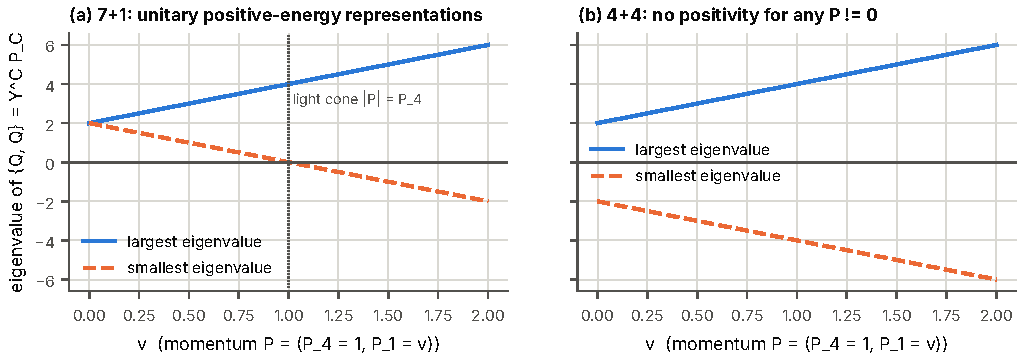
\includegraphics[width=0.92\textwidth]{../figures/fig_ng_superalgebra.pdf}
\caption{Smallest and largest eigenvalue of the matrix $\sum_C\mathsf Y^C_{\rm NG}\mathcal P^{\rm NG}_C$ of the anticommutators $\{\mathcal Q^{\rm NG}_l,\mathcal Q^{\rm NG}_{l'}\}$
for the momentum with $\mathcal P^{\rm NG}_4=1$ and $\mathcal P^{\rm NG}_1=v_{\rm NG}$, all other components zero.
(a) $7+1$: both are positive inside the light cone $v_{\rm NG}<1$. (b) $4+4$: the smallest is negative for
every momentum. Data: \texttt{data/ng\_superalgebra\_positivity.csv}.}
\label{fig:susy}
\end{figure*}

\subsection{Tensorial charges: a McGlinn-type counterexample}

On $7+1$ the matrix $C^+_{1671}\gamma^K_{1671}$ is symmetric exactly when the number $r$ of indices in
$K$ is 0, 1, 4, 5 or 8, because transposition reverses the order of the factors; their numbers
$1+8+70+56+1=136$ add up to the dimension of the space of symmetric $16\times16$ matrices. The most
general anticommutator therefore is
\begin{align}
\{\mathcal Q^{\rm NG}_l,\mathcal Q^{\rm NG}_{l'}\}&=\sum_C(\mathsf Y^C_{\rm NG})_{ll'}\mathcal P^{\rm NG}_C\nonumber\\
&\quad+\sum_{K:\,r\in\{0,4,5,8\}}(C^+_{1671}\gamma^K_{1671})_{ll'}\,\mathcal Z^K_{\rm NG},
\label{eq:tensorial}
\end{align}
with 128 \emph{tensorial charges} $\mathcal Z^K_{\rm NG}$ that commute with the momenta and the
supercharges, and on which the Lorentz generators and the R-charge act as the graded Jacobi identity
dictates (the program determines these actions from it). The extended algebra of 181 generators
satisfies the graded Jacobi identity on all {{GEN:susy_triples_ext}} triples (check S-2b). Of the
charges, the 126 with four or five indices commute with all momenta but are \emph{not} Lorentz
scalars, and 72 (those with 0, 4 or 8 indices) carry R-charge (check S-3). Generators that commute
with the translations but not with the Lorentz group are what McGlinn's theorem excludes when they
form a semisimple algebra; these form an abelian algebra, so its hypothesis H6 fails. In a theory of
particles alone such charges must vanish~\cite{HLS1975}; they are carried by extended objects.
